\part{Teoretická část}

\chapter{Rozdělení pojmu XR}

\gls{xr} je pojem zastřešující tři různá odvětví \poml \gls{vr} (Virtual Reality), \gls{ar} (Augmented Reality) a \gls{mr} (Mixed Reality). Každé funguje na principu úpravy člověkem vnímané reality, ale přistupuje k~němu jinak.

Virtuální realita (\gls{vr}) označuje typ rozšířené reality, ve kterém je uživatel pomocí headsetu kompletně přenesen do virtuálního světa, prvky z~fyzického světa vůbec nevidí a neinteraguje s~nimi. Příklady zařízení: \textit{HTC Vive}, \textit{Meta Quest}

Upravená (či augmentovaná) realita (\gls{ar}) označuje typ rozšířené reality, ve kterém uživatel vidí virtuální předměty ve fyzickém světě. AR nemusí nutně vyžadovat speciální hardware. Příklady zařízení: mobilní telefony, kapesní herní konzole

Smíšená realita (\gls{mr}) označuje typ rozšířené reality, ve kterém uživatel vidí virtuální předměty ve fyzickém světě, přičemž fyzický svět a virtuální svět mezi sebou vzájemně interagují. Příklady zařízení: \textit{Apple Vision Pro}, \textit{Meta Quest Pro} \cite{xr_disambiguation}

\chapter{Historie XR}

\section{Počátky XR}

První pokusy o~rozšířenou realitu pochází už z~50. let 20. století, kdy \textit{Morton Hellig}, americký kinematograf, přivádí na svět své zařízení zvané \textit{Sensorama}. Nejednalo se ovšem o~headset, který si vybavíme dnes \poml \textit{Sensorama} bylo stacionární zařízení, vzhledově připomínající herní automat. Hellig toto zařízení nazýval \uv{zážitkovým divadlem}, které bylo schopné zobrazit 3D obraz, pouštět stereo zvuk a vytvářet vítr. Tím se od dnešní XR technologie zásadně liší; nepřijímá vstup uživatele. \textit{Sensorama} se ovšem nedočkala úspěchu a známe ji jen jako historicky první pokus o~virtuální realitu. \cite{otechnice}

Dalším průkopníkem rozšířené reality je \textit{Ivan Sutherland}, americký vědec, který je často označován jako otec počítačové grafiky. Ve svém díle \textit{The Ultimate display} (ultimátní displej) popsal virtuální realitu tak, jak ji známe dnes. Představoval si ji jako helmu, do které odesílá obraz počítač v~reálném čase. Uživatel se tak měl ocitnout ve fiktivním světě nerozpoznatelným od světa reálného. \cite{otechnice} \cite{ivan_sutherland_bio}

Tuto představu se Sutherland snažil realizovat se svými studenty. Společně vynalezli vůbec první headset pro virtuální realitu, zvané \textit{The Sword of Damocles} \poml česky Damoklův meč. Vzhledem k~jeho primitivnosti zobrazovalo pouze čtvercové místnosti tvořené z~čar, které software následně transofrmoval do správné perspektivy. Pohyby sledovalo pomocí mechanického ramene připevněného ke stropu, ze kterého byl headset zavěšený. \cite{otechnice} \cite{Rheingold_1992}

\section{XR v~armádě}

V~80. letech 20. století o~XR projevila zájem armáda USA, ve snaze snadněji a efektivněji připravit americké piloty na ovládání letadel. Začala využívat speciálních simulačních kabin, které obsahovaly mimo jiné i speciální headset. Tento headset pomocí stereoskopického zobrazení informoval o~průběhu letu, zobrazoval 3D mapy a snímky z~radaru. Díky možnosti systém ovládat pomocí hlasu nebo pohybu očí se tento headset přibližuje k~dnešnímu stavu VR, jelikož reaguje na vstup uživatele. \cite{otechnice}


\begin{figure}[H]
    \centering

    \begin{minipage}{.5\textwidth}
        \centering
        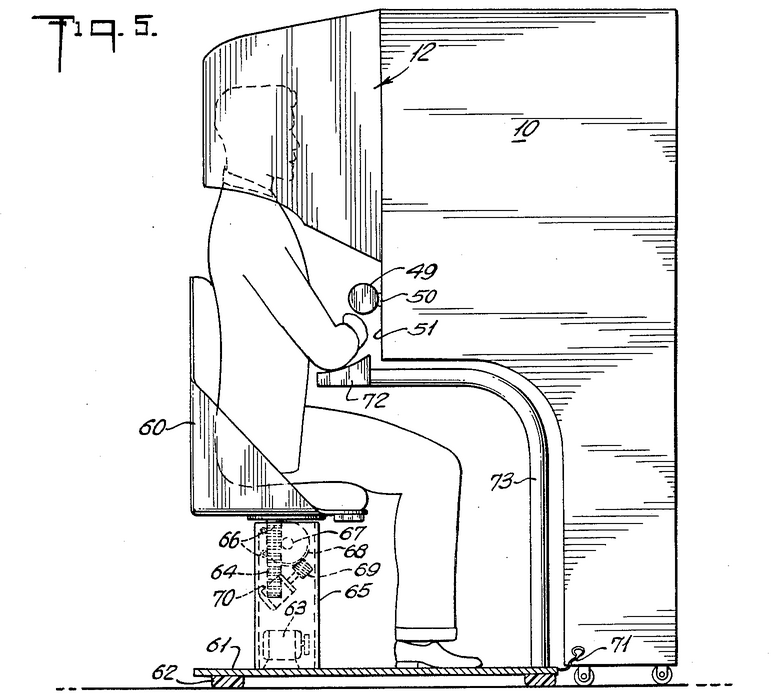
\includegraphics[height=120pt]{sensorama.png}
        \caption{Sensorama \cite{sensorama_patent}}
        \label{sensorama_fig}
    \end{minipage}%
    \begin{minipage}{.5\textwidth}
        \centering
        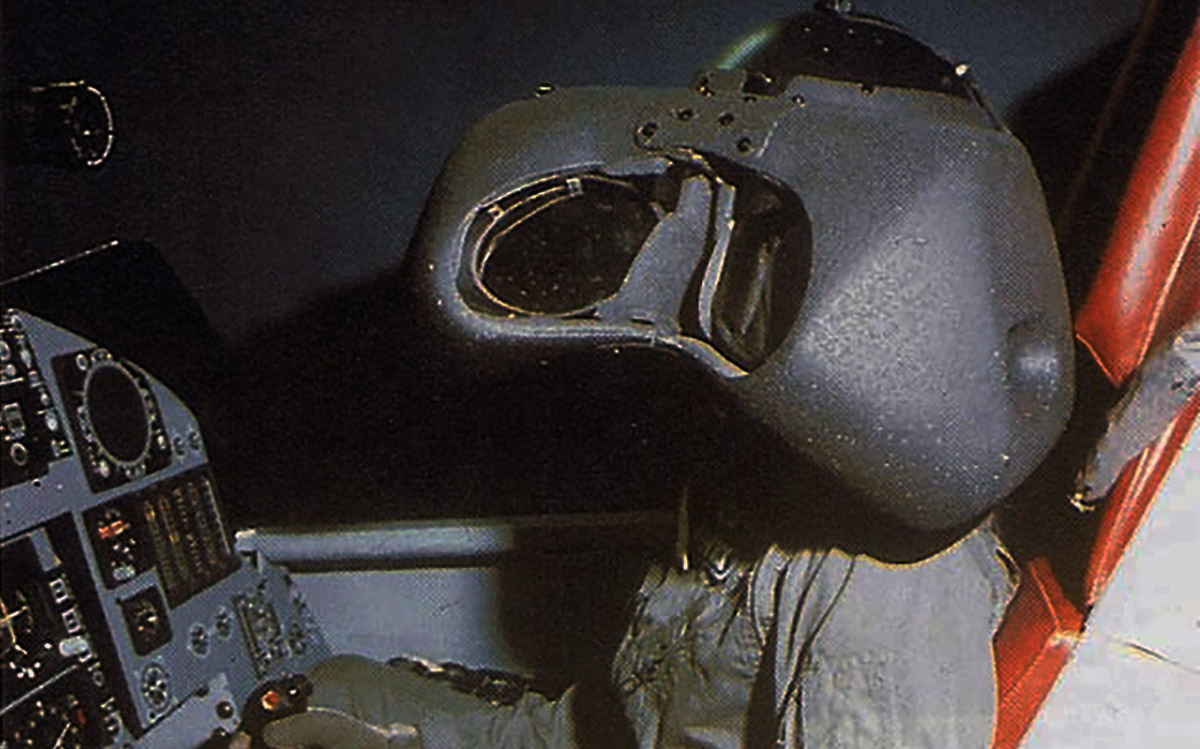
\includegraphics[height=120pt]{super_cockpit_helmet.jpg}
        \caption{Helma \textit{Darth Vader}, jedna z~částí simulačního kokpitu \cite{super_cockpit_image}}
        \label{sensorama}
    \end{minipage}

\end{figure}

\section{Komerční dostupnost}

O~počátku dostupnosti XR zařízení můžeme mluvit v~90. letech 20. století, kdy se tato technologie mohla dostat i do rukou obyčejných lidí. Dvojice zaměstnanců herní společnosti \textit{Atari}, \textit{Jaron Lanier} a \textit{Thomas Zimmermann}, společně založili společnost \textit{VPL Research} a začali s~vývojem produktů pro XR. Zaměřili se na výrobu speciálních obleků a rukavic, které dokázaly přenést pohyby uživatele do počítače. Snímání pohybu ale nebylo dostatečně kvalitní a úspěch nezaznamenalo; dodnes je ovšem známé jako první cenově dostupný XR systém. \cite{otechnice_2}

Herní společnosti na sebe také nenechaly dlouho čekat a začaly s~vývojem VR konzolí pro hraní VR her. První takovou byla britská společnost \textit{Virtuality}, která v~roce 1991 uvedla na trh stejnojmenné zařízení představující arkádový stroj se stereoskopickými brýlemi. Kvůli vysoké pořizovací ceně nebylo dostupné pro domácnosti, Virtuality ovšem otevřela nespočet heren po celé Velké Británii. \cite{otechnice_2} \cite{independent_virtuality}

Do světa VR herních konzolí vstoupily i dnes stále známé japonské společnosti \textit{SEGA} a \textit{Nintendo}, se svými \textit{SEGA VR} a \textit{Virtual Boy}. Obě tato zařízení však byla komerčními selháními. SEGA byla nucena kvůli technickým problémům vydání několikrát posunout a krátce po vydání skončila jeho výrobu. Nintendo sice své zařízení vydalo, ale rok po uvedení na trh jej stáhlo. Kvůli vysoké ceně a špatným grafickým schopnostem (konzole uměla zobrazit pouze červenou a černou barvu) si zálibu u~hráčů nenašlo.\cite{otechnice_2}

\begin{figure}[H]
    \centering
    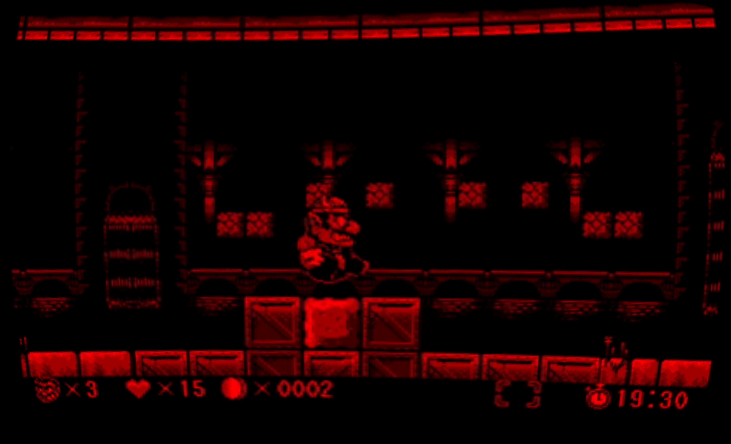
\includegraphics[height=120pt]{vboy.png}
    \caption{Červeno\textendash černé zobrazení zařízení Virtual Boy \cite{vboy}}
    \label{vboy_red_display}
\end{figure}

\section{XR dnes}

Současná generace XR zařízení se začíná objevovat po roce 2010. Velkým průkopníkem v~oblasti virtuální reality byla americká společnost \textit{Oculus}, která oznámila zájem o~vytvoření moderního VR systému. Jejich kickstarter\footnote{\url{https://kickstarter.com/}; webová stránka, kde začínající společnosti můžou žádat o~finanční podporu veřejnosti. V~Česku je známou alternativou \em Startovač (\url{https://startovac.cz/})} se ukázal jako úspěch a přilákal pozornost jiných společností, zejména tehdejšího \textit{Facebooku} (dnes \textit{Meta}). Ten společnost Oculus odkoupil ještě před tím, než stačila vydat své první zařízení. Na to si zájemci museli počkat až do roku 2016, ve kterém byl vydán headset \textit{Oculus Rift CV1}. Jeho konkurencí byl \textit{HTC Vive} od tchajvanské společnosti \textit{HTC}. Tato zařízení fungovala pouze při propojení s~počítačem; nebyla tedy samostatná. \cite{otechnice_3}

Vývoj mobilního VR (tedy takového headsetu, který nepotřebuje počítač pro vykreslování obsahu) společnost Oculus konala za podpory korejského Samsungu, se kterým na trh uvedla \textit{Gear VR} \poml headset, který pro vykreslování používal mobilní telefon. Na podobném principu fungoval i experiment od Googlu zvaný \textit{Cardboard VR}. Ten pro virtuální realitu používal pouze mobilní telefon a headset složený z~kartonu (odtud název). Mobilní VR se v~této době neuchytilo, zažilo ovšem velký rozmach v~letech 2019\textendash2020 po vydání headsetu \textit{Oculus Quest} (dnes \textit{Meta Quest}), který byl plně samostatný a používal upravenou verzi OS Android. Hry pro tento headset jsou upravené, aby běžely na Androidu, nicméně existuje možnost jej připojit k~počítači a hrát hry pro \uv{nesamostatné} headsety. \cite{otechnice_3}

Díky technologickým pokrokům a zmenšování hardwaru se také začala objevovat zařízení pro smíšenou realitu, která pomocí snímačů a pohledu z~kamery umožnila vkládat virtuální předměty do reálného světa. Forem měla mnoho; například upravené optické brýle s~malým displejem nebo speciální průsvitný headset. Prorazit s~těmito zařízeními se pokoušeli technologičtí giganti jako Google a Microsoft. Kvůli vysokým pořizovacím cenám ale tato zařízení u~jednotlivců neuspěla a tyto společnosti s~nimi dodnes cílí na pracovní prostředí. \cite{google_glass_mobilenet}

Velmi dostupné byly naopak aplikace používající augmentovanou realitu. AR byla integrována do již existujících zařízení, především jako technická demonstrace. Zpočátku bylo běžné AR realizovat pomocí speciálních předmětů či kartiček, kvůli jednoduchosti. Zařízení tento předmět rozpoznalo, určilo jeho otočení a naklonění, a následně zobrazilo obsah navrch. Zlom nastal, když Google vydal \textit{ARCore}, \gls{SDK} pro AR, který umožnil vývojářům sledovat pohyb mobilního telefonu pouze pomocí pohledu z~kamery. Vývojáři se tím pádem mohli zaměřit pouze na vývoj jejich aplikací a her, jelikož nemuseli investovat čas a peníze do technologie sledování pohybu. Právě v~této době vznikla většina aplikací a her, které známe. Za zmínku stojí například \textit{Pokémon GO}. \cite{enwiki:1182789097}

\chapter{Hardware}

\section{Degrees of freedom}

Hlavním tématem, kterým se XR liší od tradičních výpočetních zařízení, je sledování pohybu. S~tímto je také spojen pojem \textit{Degrees of freedom} (DoF), česky volně přeloženo jako \textit{stupně volnosti}. Ten označuje počet směrů, kterým se předmět může pohybovat \poml buď po ose, nebo kolem ní. V~našem trojrozměrném světě se můžeme pohybovat v~6 směrech. \cite{mechatech_3dof_6dof}

\begin{figure}[H]
    \centering
    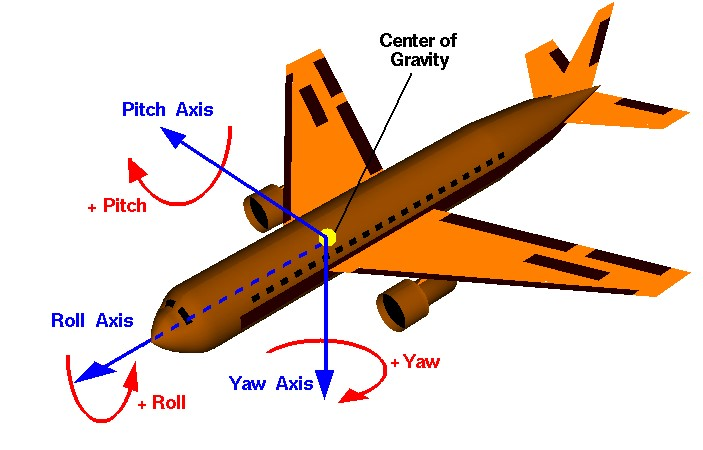
\includegraphics[height=150pt]{rotations.jpg}
    \caption{Diagram zobrazující 6 možných pohybů v~3D prostoru \cite{nasa_aircraft}}
    \label{rotations_nasa_fig}
\end{figure}

V~XR rozlišujeme 3DoF (3 stupně volnosti) a 6DoF (6 stupňů volnosti). Zařízení, které sleduje uživatelův pohyb ve 3DoF, umí rozpoznat pouze náklon či otočení. Umožňuje tak se otáčet a rozhlížet ve virtuálním prostoru. Avšak zařízení, které sleduje pohyb v~6DoF, je kromě toho schopné sledovat také pohyb dopředu/dozadu, doleva/doprava a nahoru/dolů. Umožňuje tak se ve virtuálním prostoru \textit{pohybovat}, tedy nebýt jen pozorovatelem. \cite{mechatech_3dof_6dof}

Pro sledování náklonu a pohybu se používají odlišné technologie, které popisuji v~následujících částech.

\section{Gyroskop}

Gyroskop je elektronické zařízení, které umožňuje vypočítat úhlové zrychlení. Jejich zpracování jsou různá, v~spotřebitelské elektronice převažují \textit{vibrační gyroskopy}, díky malým rozměrům, ceně a dostatečné přesnosti. V~součástce je rozkmitáno malé těleso, na které je vlivem otáčení vyvinuta Coriolisova síla, která působí kolmo na osu otáčení. Tato síla je úměrná rychlosti otáčení a jejím změřením můžeme určit rotaci zařízení. \cite{Electricity_Magnetism} \cite{techmania_coriolis}

\section{Sledování pohybu}

Sledování pohybu v~prostoru je řešeno různými způsoby. Podle postavení zařízení je možné je seskupit do dvou kategorií: vnější sledování (outside-in) a vnitřní sledování (inside-out).

Vnější sledování využívá speciální zařízení (\uv{věže}) rozmístěná v~prostředí, ve kterém je sledován pohyb. Taková zařízení mohou být např. emitery infračerveného světla, které sledované zařízení zaznamená a vypočítá podle nich svoji pozici v~prostoru. Protože pro sledování jsou použita tato genercká zařízení, těší se tento způsob sledování vysoké kompatibilitě \poml pro různá zařízení není potřeba pořizovat jiné věže (za předpokladu, že toto nové zařízení také využívá vnějšího sledování). Nevýhodou je naopak obtížná přenosnost takového systému. \cite{vr_tracking_suvi}

Vnitřní sledování se v~dnešní době stává populárnějším. Na rozdíl od vnějšího sledování nevyužívá žádných externích zařízení a je úplně samostatné. První takový systém představil Google se svým ARCore, zmíněným v~předchozí kapitole. Ten umožnil sledování pozice pouze pomocí pohledu z~kamery. Protože je ale navržen pro spuštění na většině mobilních zařízení, výsledky jsou poněkud nekonzistentní (kvůli lišícím se kvalitám kamer).
Revoluci v~tomto odvětví způsobila společnost Meta se svým inovativním řešením. Používá sadu čtyř kamer, které průběžně sledují a analyzují prostor kolem uživatele. V~tomto prostoru si poté vytvoří záchytné body, jejichž pozici analyzuje použitím AI algoritmů. Tímto je takový systém velice přenosný a pro běžného uživatele neuvěřitelně přesný. V~nevhodném prostředí tento systém ale přestává fungovat (např. v~špatných světelných podmínkách). \cite{vr_tracking_suvi} \cite{enwiki:1182789097}

\section{Stereoskopické zobrazení}

V~oblasti \gls{vr}, případně \gls{mr} je klíčovým prvkem stereoskopické zobrazení. V~principu headset každému oku zobrazuje jiný obraz, což vyvolává pocit hloubky a dělá tak VR přesvědčivou. Renderování tedy musí proběhnout dvakrát, pokaždé pod jiným úhlem. \cite{stereoskopie_diagram}

\begin{figure}[H]
    \centering
    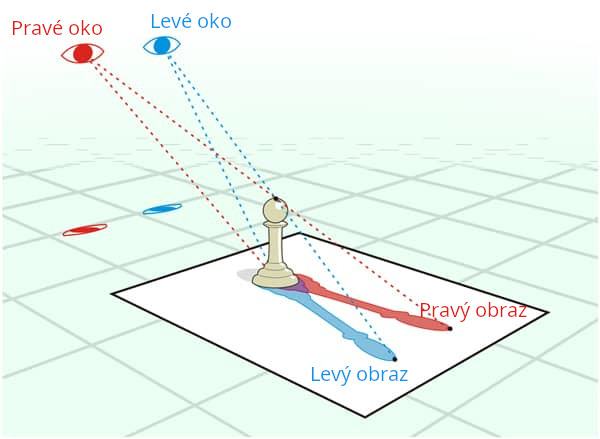
\includegraphics[height=180pt]{depth-perception.jpg}
    \caption{Podstata stereoskopického zobrazení \cite{stereoskopie_diagram}}
    \label{depth_perception}
\end{figure}

Stereoskopie ovšem nemá použití pouze ve VR. Široké využití nachází i ve filmařství, při promítání 3D filmů. Pomocí speciálních polarizačních brýlí je promítaný obraz rozdělen na dva odlišné obrazy, pro levé a pravé oko. \cite{unitedfilm_stereoskopie}

Existují také \textit{autostereoskopické displeje}, které obraz rozdělí pomocí tzv. \textit{paralaxové bariéry}. Tuto technologii využila společnost Nintendo ve své herní konzoli \textit{Nintendo 3DS}. \cite{enwiki:1158939127}

\chapter{Software}

V~dnešní době, díky standardizovaným rozhraním, je vývoj pro XR mnohem jednodušší než kdysi. S~vydáním prvních komerčních VR zařízení se začínaly formovat první \gls{SDK} pro virtuální realitu. V~principu výrobce při vývoji zařízení stanoví rozhraní, přes které software komunikuje s~hardwarem. 

Například Oculus se svým zařízením Oculus Rift přišel se svým vlastním řešením, \textit{Oculus SDK}, jehož použití bylo bezplatné a bylo integrováno do většiny herních enginů. \cite{enwiki:1193283032} Toto ale přispělo k~fragmentaci XR ekosystému \poml aplikace vyvinuté pro jednu platformu bylo obtížné spustit na konkurenční platformě.

Této fragmentaci se snažila zabránit americká společnost \textit{Valve}, provozovatel známé herní platformy \textit{Steam}. Ve spolupráci s~výrobci vytvořila otevřený standard \textit{OpenVR}, který vývoj VR aplikací značně usnadnil. Vývojáři nyní mohli vyvíjet pro jeden standard a zpřístupnit jejich aplikace na všech zařízeních, která implementovala toto jednotné rozhraní. OpenVR se stalo výchozím rozhraním pro headset Vive od společnosti HTC. \cite{enwiki:1192992480}

Dnes nejpoužívanějším standardem, který sjednocuje vývoj XR aplikací, je \textit{OpenXR}. OpenXR je, jako OpenVR, otevřeným standardem, který vyvíjí konsorcium \textit{Khronos Group}, které je taktéž známé pro standardy \textit{OpenGL} a \textit{Vulkan}. Toto rozhraní implementuje většina dnešních XR platforem, včetně mobilních VR headsetů založených na OS Android. OpenXR tímto vyřešilo fragmentaci v~XR systémech. \cite{enwiki:1186405367}

XR se, v~omezené podobě, dostalo i do dnešních internetových prohlížečů. Prohlížeče založené na Chromium těží ze standardu \textit{WebXR}, který přináší XR do JavaScriptu. Vývojáři tak můžou do svých webových stránek vkládat např. virtuální prohlídky. \cite{webxr_mdn}

\section{Herní engine}

Jako herní engine označujeme software, který usnadňuje vývoj her. Zpravidla obsahuje mnohé předem vytvořené nástroje pro snadnější práci s~grafikou, zvukem, fyzikou a dalšími koncepty. Vývojáři tyto funkce pak nemusí sami implementovat ve svých hrách. Jednou z~oblastí, kterou může herní engine usnadňovat, je právě podpora OpenXR. Nejznámější enginy, například Unity a Unreal Engine, podporu pro XR nabízejí už několik let. \cite{enwiki:1186405367}

Svůj vlastní projekt, který detailně popisuji v~praktické části, jsem chtěl také vyvinout v~herním enginu. Zvolil jsem si svobodný Godot Engine.

\section[Godot Engine]{Godot Engine \protect\footnote{\url{https://godotengine.org/}}}

\textit{Godot} je svobodný (open-source) herní engine, který je nabízen zdarma. Hlavní důvod, proč jsem si jej vybral namísto známějších Unity nebo Unreal Engine, je jeho licence. Godot je šířen pod svobodnou licencí MIT, která vývojářům dovoluje kód používat komerčně i nekomerčně, a to pod jedinou podmínkou: text licence je ve výsledné práci zachován. Jiné enginy jsou naopak distribuovány pod nesvobodnou licencí a za některé jejich funkce můžou od vývojářů vyžadovat poplatek.

Godot se v~poslední době stává více a více populárním a obdržel investice od významných technologických společností. Mezi ně patří např. grant od Epic Games pro vývoj grafiky a grant od Meta pro vývoj XR nástrojů. \cite{godot_epicgames} \cite{godot_meta}

Pro úpravu Godot projektů používáme oficiální editor. Základními stavebními bloky enginu jsou \textit{uzly}, které jsou uspořádány do stromu, podobně jako jsou webové stránky reprezentovány stromem značek. Tyto uzly samy o~sobě nemají mnoho funkcí, jejich kombinací ale můžeme dosáhnout komplexnějšího chování. Jednotlivé uzly se dají přirovnat k~třídám v~objektově orientovaném programování, které se navzájem rozšiřují.

Například uzel \texttt{Node3D} disponuje atributem \texttt{position} (pozice) a uzel \texttt{Camera3D}, který rozšiřuje \texttt{Node3D}, disponuje atributy \texttt{position} a \texttt{fov} (\textit{field of view}; zorný úhel). Dceřinné uzly zároveň dědí atributy rodičovských uzlů, pokud oba rozšiřují společný uzel (pokud je např. \texttt{Camera3D} dceřinný uzel \texttt{Node3D}, pak se \texttt{Camera3D} pohybuje společně s~\texttt{Node3D} (sdílí atribut \texttt{position}) a \texttt{position} na \texttt{Camera3D} je relativní posun od \texttt{Node3D})

Uzlům můžeme přiřadit \textit{skript}, který upravuje jejich chování. Tento skript se chová jako třída v~objektovém programování, která rozšiřuje daný uzel. Pokud rozšiřujeme uzel pro 2D grafiku, můžeme metodou získat pozici jako 2D vektor. Pokud rozšiřujeme uzel pro 3D grafiku, stejnou metodou můžeme získat pozici jako 3D vektor. Stejně tak můžeme přepisovat virtuální funkce. Projekty v~Godotu používají dedikovaný jazyk zvaný GDScript, existuje ale oficiální podpora jazyka C\# a komunitně vytvořená rozšíření pro Rust.

Uzel a jeho dceřinné uzly společně s~přiřazenými skripty můžeme dále uložit jako izolovanou \textit{scénu} (soubor .tscn), kterou můžeme poté \textit{instancovat}. Scéna se pak chová jako samostatný uzel. Jedna scéna je vždy hlavní scénou a je otevřena při spuštění projektu.

\begin{figure}[H]
  \centering
  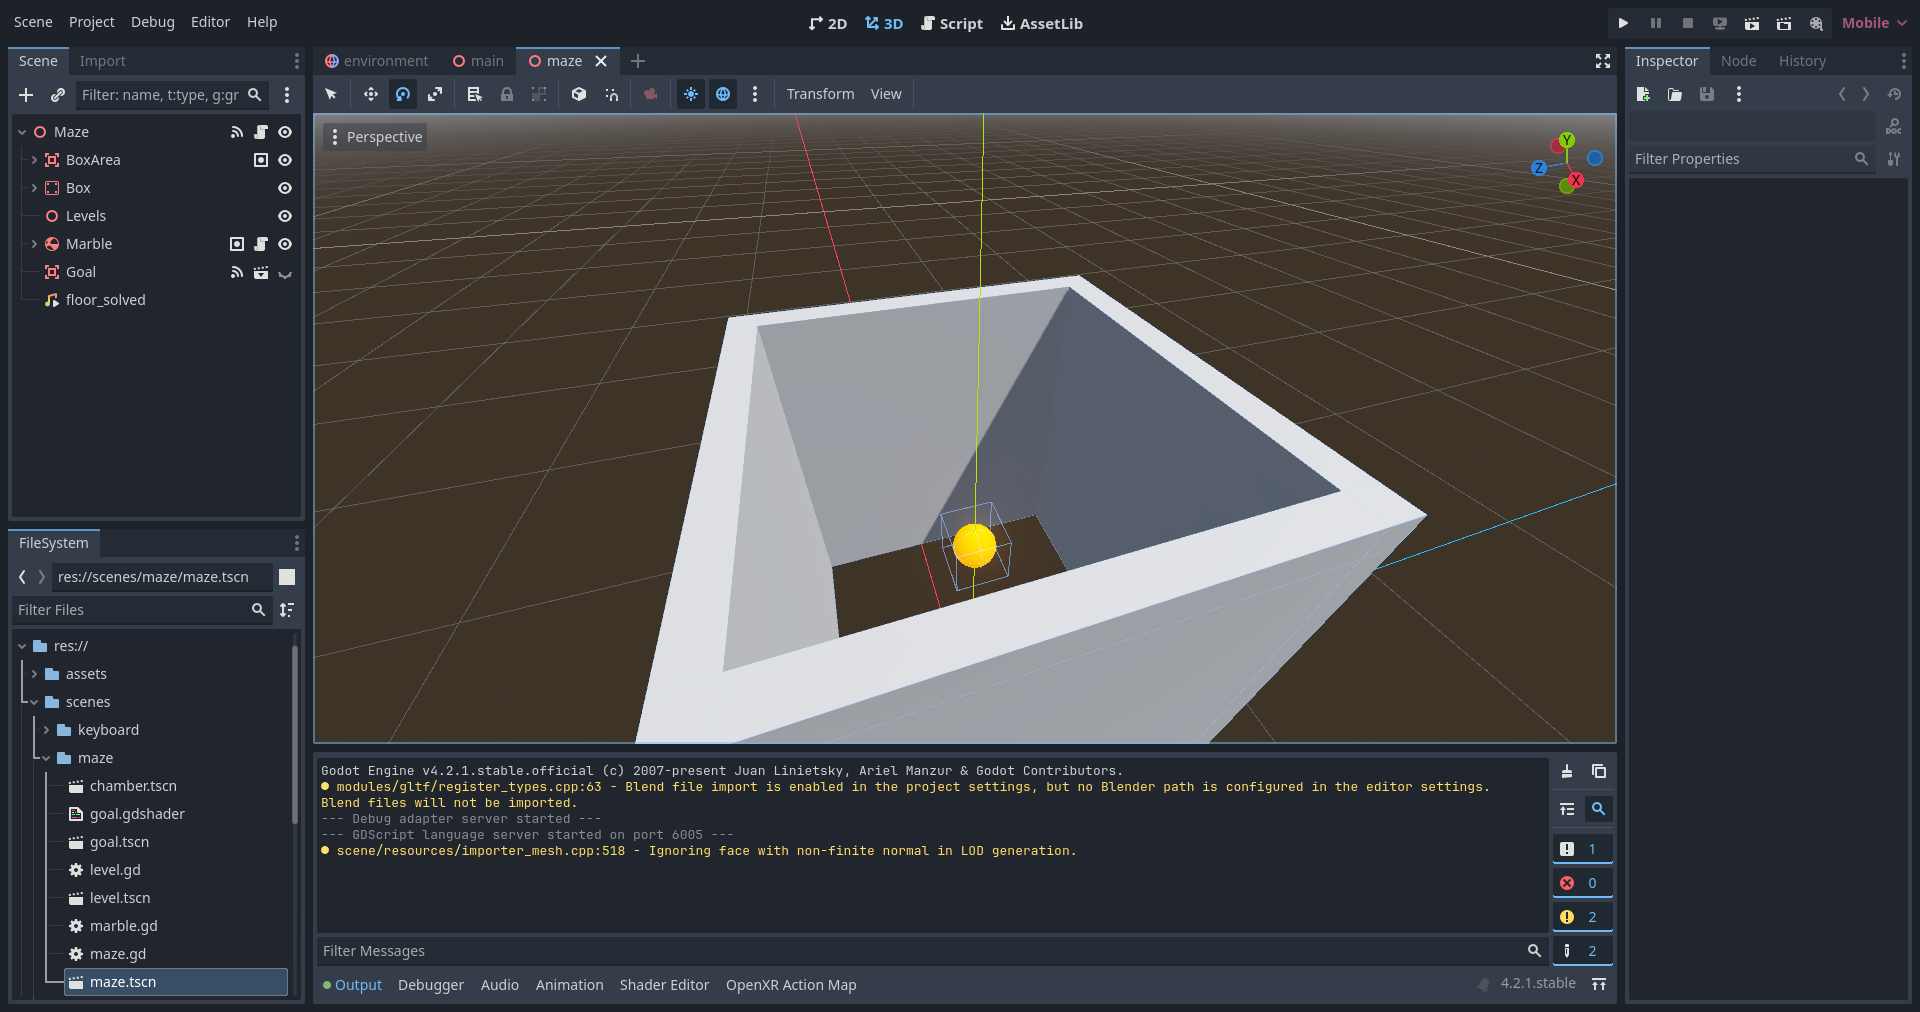
\includegraphics[height=180pt]{godot_editor.png}
  \caption{Editor Godot Engine a otevřená scéna \texttt{Maze.tscn}}
  \label{godot_editor_maze_tscn}
\end{figure}

\subsection{Jazyk \textit{GDScript}}

GDScript je jazyk, ve kterém se vyvíjí většina Godot projektů. Můj projekt je taktéž psán v~GDScriptu a z~tohoto důvodu jej zde popisuji pro snadnější pochopení kódu.

GDScript je vysokoúrovňový, objektově orientovaný, imperativní a hybridně (staticky i dynamicky) typovaný jazyk. Vzhledově nápadně připomíná jazyk Python a podobně jako Python používá odsazení pro vyjádření řídící struktury. Nabízí širokou škálu vestavěných tříd pro manipulaci dat typických pro hry, matematiku a fyziku (textury, vektory, matice) a samozřejmě obecné typy (celé číslo, desetinné číslo, textový řetězec atd.). Proměnné programátor může anotovat typem. Podporuje koprogramy (\textit{coroutines}) a událostmi řízené programování pomocí \textit{signálů}. Pro svou hlubokou integraci se samotným enginem je vhodný pro jednoduché projekty, kvůli své dynamičnosti ovšem nenabízí stejnou rychlost jako kompilované jazyky. \cite{gdscript_reference}

Pro příklad kódu v~GDScriptu nahlédněte do přílohy \ref{apx_gscript_sample}.